
\section{Theorie}
\label{sec:Theorie}

\subsection{Das Vakuum}

Ein Vakuum ist ein Raum in dem keine oder sehr wenige Teilchen enthalten sind, sodass ein hindurch fliegendes Teilchen näherungsweise keine Wechselwirkungen (Stöße) mit seiner Umgebung erfährt. Das wird durch die mittlere freie Weglänge beschrieben, die angibt welche Strecke ein Teilchen in einem Medium zurücklegen kann ohne mit diesem zu Stoßen. Benötigt wurde ein Vakuum beispielsweise in frühen Glühlampen. In der Physik findet es viele Anwendungen vor allem in Teilchenbeschleunigern damit die dort beschleunigten Teilchenpakete nicht durch Kollisionen mit Gasteilchen verloren gehen.
Ein vollkommenes Vakuum zu erzeugen ist nicht möglich, doch es gibt Pumpen die Vakuen verschiedener Reinheit erzeugen können. Das Ergebnis hängt von der Qualität des Rezipienten ab. Abgesehen von fehlender Abdichtung der Ventile und Pumpen, gibt es virtuelle Lecks, die nicht von undichten Stellen herrühren sondern bau- und lagerungsbedingt bei einem Rezipienten auftreten. Sie entstehen dadurch, dass Gase, die sich an den Innenwänden des Rezipienten angelagert haben, wieder entweichen (Desorption) oder das bei der Herstellung mit Gasen gefüllte Hohlräume entstanden sind, die durch die Wände in den zu evakuierenden Raum diffundieren.

\subsection{Arten der Vakuumerzeugung}

Grundsätzlich lassen sich diese Vakuumpumpen in zwei Kategorien einteilen.
Bei Speicherpumpen wird das im Rezipienten befindliche Gas in einem mit der Pumpe verbundenen Behältnis oder Medium zwischengespeichert, weshalb auf Grund der begrenzten Kapazität nur kleinere Gasmengen abgepumpt werden können.
Bei Transportpumpen hingegen wird das Gas über die Pumpe in die Außenluft abgeleitet. Sie lassen sich deshalb für beliebig große Gasmengen verwenden.\cite{Jena} 
Außerdem lassen sie sich in zwei Pumpentypen aufteilen:\newline
Bei einer Verdrängerpumpe wird das gas zunächst in einen abgeschlossenen Kolben gesaugt und anschließend an die Außenluft abgegeben.\newline
Kinetische Vakuumpumpen beschleunigen das Gas mittels mechanischer Arbeit oder eines gerichteten Dampfstrahls in Pumprichtung\cite{Pfeiffer}.
Die in diesem Versuch betrachteten Drehschieber- und Turbomolekularpumpe sind kinetische Vakuumpumpen.

\subsubsection{Die Drehschieberpumpe}

Eine Drehschieberpumpe besteht wie in Abbildung \ref{fig:DSP} zu sehen aus einer zylindrischen Pumpkammer(1), einem zylindrischen Rotor(2), durch Feder an die Wand gedrückte Drehschieber, die die Kammer in zwei Halbräume teilt, und einem Ablassventil(4). Aus dem Rezipienten(R) strömt das Gas in die Kammer, wird komprimiert und durch den Überdruck am Ventil an die Außenluft abgegeben.\cite{Jena}
So kann ein Rezipientengasdruck $p\approx \SI{0,5e-1}{\milli\bar}$ (Feinvakuum) erzeugt werden.
In diesem Druckbereich liegt eine viskose laminare Strömung des abgepumpten Gases vor, dass heißt auf Grund der großen Teilchenzahlen stoßen diese fast nur untereinander und kaum mit den Innenwänden er Pumpenrohre. Deren Durchmesser kann deshalb gering gewählt werden.
\begin{figure}
\centering
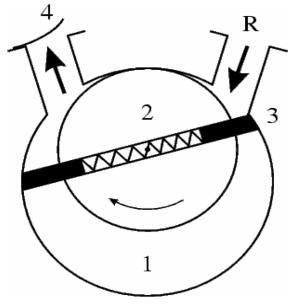
\includegraphics[scale=0.3]{content/images/Drehschieber.jpg}
\caption{Schematischer Aufbau einer Drehschieberpumpe \cite{Jena}.}
\label{fig:DSP}
\end{figure}

\subsubsection{Die Turbomolekularpumpe(Turbopumpe)}

Bei einer Turbopumpe ähnelt der Rotor einer mehrstufigen Turbine mit schaufelähnlichen Scheiben, während zwischen den Rotorscheiben spiegelverkehrte Schaufeln fest angebracht sind.
Der Rotor ist meist auf der Vorvakuum-Seite der Kammer auf einem Kugellager und auf der Hochvakuum-Seite auf einem verschleißfreien Permanentmagnetlager gelagert, um Verunreinigungen es Vakuums durch Schmierstoffe zu vermeiden.\cite{Pfeiffer} Aufgrund der hohen Drehzahl des Rotors können mit einer Turbopumpe Enddrücke bis $p=\SI{1e-11}{\milli\bar}$(Ultrahochvakuum) erreicht werden, allerdings benötigt sie bereits ein Feinvakuum um zu arbeiten. Außerdem werden für den Hochvakuumbereich dickere Rohre benötigt, da dort eine molekulare Strömung vorliegt, also die wenigen verblieben Teilchen fast ausschließlich zwischen den Rohrwänden hin und her prallen und somit die mittlere freie Weglänge viel größer ist als der Rohrdurchmesser.

\subsection{Das Saugvermögen}
Die Pumpen werden durch ihr Saugvermögen 
\[
S=\frac{\mathrm{d}V}{\mathrm{d}t}
\]
charakterisiert.
Es beschreibt den durch die Ansaugöffnung der Pumpe fließenden Volumenstrom und kann über verschiedene Methoden gemessen werden.

\subsubsection{Messung der p(t)-Kurve}
Nach dem Boyle'schen Gesetz für ideale Gase gilt bei einer konstanten Temperatur $T$:
\begin{equation}
p\cdot V =\text{const}\label{eq:Boyle}
\end{equation}
Eine Ableitung nach der Zeit ergibt
\[
\frac{\mathrm{d}V}{\mathrm{d}t} = S = - \frac{V}{p} \frac{\mathrm{d}p}{\mathrm{d}t}
\]
Nach $p$ auflösen ergibt schließlich
\begin{equation}
p(t)=p_.0\exp{-\frac{S}{V_.0}t}\label{eq:pt1}
\end{equation}
und unter  Berücksichtigung, dass nie ein vollständiges Vakuum erreicht wird und ein Enddruck $p_.E$ verbleibt,
\begin{equation}
p(t)=(p_.0-p_.E)\exp{-\frac{S}{V_.0}t}+p_.E\text{.}\label{eq:pt2}
\end{equation}

\subsubsection{Leckratenmessung}
Wenn der Enddruck $p_.E$ erreicht ist, stellt sich ein Gleichgewicht ein. Es strömt durch (virtuelle) Lecks 
genau soviel Gas in den Rezipienten wie die Pumpe absaugen kann.
Wird die Pumpe in diesem Zustand abgeschaltet, füllt sich der Rezipient langsam wieder mit Gas und es gilt 
\[
S=\frac{Q}{p_.E}\text{.}
\]
Die Zählrate $Q$ bestimmt sich mit der Druckänderung $\Delta p$ in der Zeit $\Delta t$ nach
\[
Q=V_.0\frac{\Delta p}{\Delta t}
\]
und damit
\begin{equation}
S=\frac{V_.0}{p_.E}\cdot\frac{\Delta p}{\Delta t}\label{eq:S}
\end{equation}
\subsection{Arten der Vakuummessung}

\subsubsection{Pirani-Vakuummeter}

Das Pirani-Vakuummeter arbeitet im Feinvakuum, also für $p\approx \SI{1e-1}{\milli\bar} - \SI{1e-3}{\milli\bar}$ und nutzt, dass die Wärmeleitfähigkeit von Gasen proportional zum Druck ist. Es wird ein Draht in einer mit dem Rezipienten verbundenen Messröhre mit konstantem Strom erhitzt. Je niedriger der Druck desto weniger Wärme kann abtransportiert werden, weshalb sich der Draht weiter aufheizt, wodurch sich sein Widerstand erhöht. Über eine Wheatstone-Brücke kann dieser gemessen und so der Rezipientendruck bestimmt werden.\cite{Jena}

\subsubsection{Penning-Vakuummeter}

Das Penning- oder Kalt-Ionisations-Vakuummeter arbeitet im Hoch- und Ultrahochvakuum ($\SI{1e-3}{\milli\bar} - \SI{1e-12}{\milli\bar}$). Ein Glaskolben wird an den Rezipienten angeschlossen und durch natürliche Raumionisation freigewordene Elektronen werden zwischen zwei Elektroden beschleunigt. Sie können dabei weitere Elektronen ausschlagen, sodass der fließende Strom ein Maß für den Gasdruck ist. Durch einen am Kolben befestigten Permanentmagneten, werden die Elektronen in eine Spiralbahn ausgelenkt und so der Beschleunigungsweg zwischen den Elektroden vergrößert, um den Messbereich zu erweitern.\cite{Jena}

\subsubsection{Bayard-Alpert-Vakuummeter}

Beim Bayard-Alpert-Vakuummeter ist die Elektronenquelle eine Glühkathode. Die Elektronen werden zu der Anode hin beschleunigt und ionisieren auf dem Weg die verbliebenen Gasteilchen. Die Ionen werden zu einer weiteren negative geladenen Elektrode beschleunigt und beim Auftreffen neutralisiert, was zu einem messbaren Strom führt.\cite{Spektrum}
